\chapter{Theoretical Background}
\label{chap2}
\section{Fundamentals of Bearing Fault Frequencies}
{
\subsection{Overview}
{
The most significant challenge that the authors had to deal with is that of the faulty cases detection. For this reason, fault and unfault models have been developed, and series of comparisons between the actual model generated by apparatus measurements and these two situational models are being executed. This development constitutes a real challenge since this is the main criterion that identifies the state of the motor.
}

\subsection{Unfault and Fault Models}
{
As previously mentioned, the authors make use of a model-based approach, which entails that the main concept is comparison-oriented. Specifically, there is the unfault model, which contains a high-amplitude peak at the shaft rotating frequency $F_{\omega}$. In addition to that, it can be noticed in Figure~\ref{fig:faultsunfaults} that some other patterns distinct themselves from the previously-mentioned unfault model. Regarding the unbalance model, it is obvious that the amplitude at the first tone is much greater. In the case of the misalignment model, it can be noticed that the tone at $2F_{\omega}$ has a much greater amplitude while the amplitude at the tone of the shaft speed $F_{\omega}$ remains at a high level. In the case of looseness, there are some more tones prevailing on the spectrum, among the tones related to the shaft speed. To top it all off, the most important vibration spectrum is that of the bearing failure (Refer to Figure~\ref{fig:faultTree}). Every bearing is characterized by four critical frequencies, given by its manufacturer, and these frequencies are associated with the four bearing components (inner and outer ring, balls, and cage):

\begin{itemize}
	\item BPFO (Ball Pass Frequency Outer) - outer race failure
	\item BPFI (Ball Pass Frequency Inner) - inner race failure
	\item BSF (Ball Spin Frequency) - rolling element failure
	\item FTF (Fundamental Train Frequency) - cage failure
\end{itemize}

\begin{figure}[h]
\centering
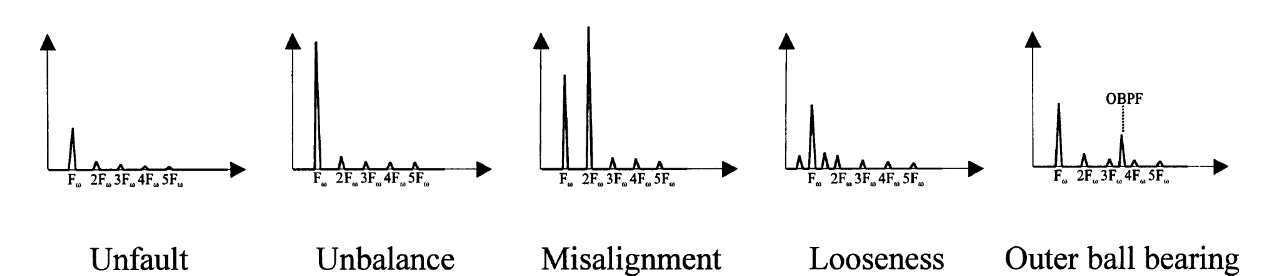
\includegraphics[width=\linewidth]{figures/FaultsAndUnfaults.png}
\caption{Fault and unfault spectrum graphs \cite{Betta2002}.}
\label{fig:faultsunfaults}
\end{figure}

The procedure to calculate critical frequencies involves two steps: first computing the bearing frequency factors, then deriving the vibration frequencies. The following analysis covers the case where the inner race rotates while the outer race remains stationary.

\begin{align}
	F_{\text{OR}} &= \frac{Z}{2} \left(1 - \frac{d}{D} \cos\alpha\right) 
	&&\text{(Outer Race Fault)} \label{eq:OR} \\
	F_{\text{IR}} &= \frac{Z}{2} \left(1 + \frac{d}{D} \cos\alpha\right) 
	&&\text{(Inner Race Fault)} \label{eq:IR} \\
	F_{\text{FTF}} &= \frac{1}{2} \left(1 - \frac{d}{D} \cos\alpha\right) 
	&&\text{(Cage Frequency, Inner Race Rotating)} \label{eq:FT} \\
	F_{\text{BS}} &= \frac{D}{d} \left[1 - \left(\frac{d}{D}\right)^2 \cos^2\alpha\right] 
	&&\text{(Ball Spin Frequency)} \label{eq:BS}
\end{align}

Then, the aforementioned factors when multiplied with shaft speed ($f$) give specific critical bearing vibration frequencies:
\begin{align}
	\text{BPFO} &= f \times F_{\text{OR}} \label{eq:BPFO} \\
	\text{BPFI} &= f \times F_{\text{IR}} \label{eq:BPFI} \\
	\text{BSF}  &= f \times F_{\text{BS}} \label{eq:BSF} \\
	\text{FTF}  &= f \times F_{\text{FTF}} \label{eq:FTF}
\end{align}

where:
\begin{align*}
	&f    &&: \text{Shaft rotational speed (\si{\hertz})} \\
	&\text{BPFI} &&: \text{Ball pass frequency, inner race} \\
	&\text{BPFO} &&: \text{Ball pass frequency, outer race} \\
	&\text{FTF}  &&: \text{Fundamental train frequency} \\
	&\text{BSF}  &&: \text{Ball spin frequency} \\
	&Z    &&: \text{Number of rolling elements} \\
	&D    &&: \text{Pitch circle diameter of the bearing (\si{\milli\meter})} \\
	&d    &&: \text{Rolling element (ball) diameter (\si{\milli\meter})} \\
	&\alpha &&: \text{Contact angle (\si{\degree})} \\
\end{align*}

It is also worth noting that the bearing frequency factors can be obtained through: 
\begin{itemize}
	\item Manufacturer-provided values
	\item Direct calculation using the above equations \eqref{eq:OR}--\eqref{eq:BS}
	\item Reverse calculation from measured vibration frequencies \eqref{eq:BPFO}--\eqref{eq:FTF}
\end{itemize}

To summarize the preceding analysis, Figure \ref{fig:faultTree} provides a clear visualization of the fault diagnosis procedure. When analysis reveals elevated frequency tones, a systematic approach must be followed to identify the source of these dominant frequencies. This process essentially involves mapping characteristic vibration patterns to specific machine faults on a frequency spectrum plot.


\begin{figure}[h]
	\centering
	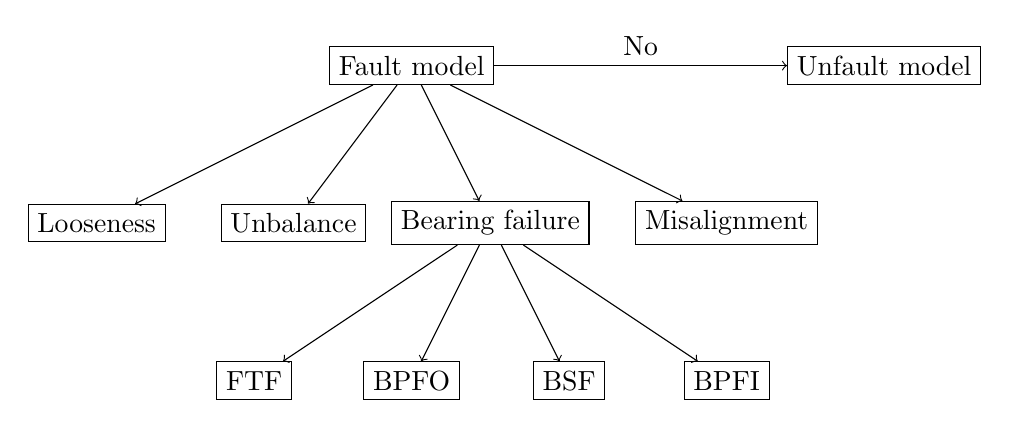
\begin{tikzpicture}[node distance=1.5cm]
		\node (box1) [draw, rectangle] at (0,0) {Unfault model};
		\node (box2) [draw, rectangle, left of=box1, node distance=6cm] {Fault model};
		\node (box3) [draw, rectangle] at (-7.5,-2) {Unbalance};
		\node (box4) [draw, rectangle] at (-2,-2) {Misalignment};
		\node (box5) [draw, rectangle] at (-5,-2) {Bearing failure};
		\node (box6) [draw, rectangle] at (-10,-2) {Looseness};
		\node (box7) [draw, rectangle] at (-6,-4) {BPFO};
		\node (box8) [draw, rectangle] at (-2,-4) {BPFI};
		\node (box9) [draw, rectangle] at (-4,-4) {BSF};
		\node (box10) [draw, rectangle] at (-8,-4) {FTF};
		
		% Arrows with labels
		\draw[->] (box2) -- node[midway, above] {No} (box1);
		\draw[->] (box2) -- (box3);
		\draw[->] (box2) -- (box4);
		\draw[->] (box2) -- (box5);
		\draw[->] (box2) -- (box6);
		\draw[->] (box5) -- (box7);
		\draw[->] (box5) -- (box8);
		\draw[->] (box5) -- (box9);
		\draw[->] (box5) -- (box10);
	\end{tikzpicture}
	\caption{Fault tree analysis diagram showing the relationship between machine conditions and specific fault frequencies.} \label{fig:faultTree}
\end{figure}

It must be that a fault-emulation method can be used in such cases to simulate the faulty models. This entails that additional tones can be stressed, and crucial spectra modifications may take place for research and comparison purposes.
}
}




\section{Algorithms and Technologies}
\subsection{Algorithm Introduction}
{
This section aims at yielding a brief introduction into the concept of bearing failure prdictive maintenance plan. The set-up utilizes an accelerometer which collects data that are going to be used for model assessment, by the means of Fast-Fourier Analysis.

In most of the actual applications a machine learning implementation is a common practice. A figure that depicts this modeling has been presented by Dharmarathne et al \cite{Dharmarathne2025}.

\begin{figure}[h]
	\centering
	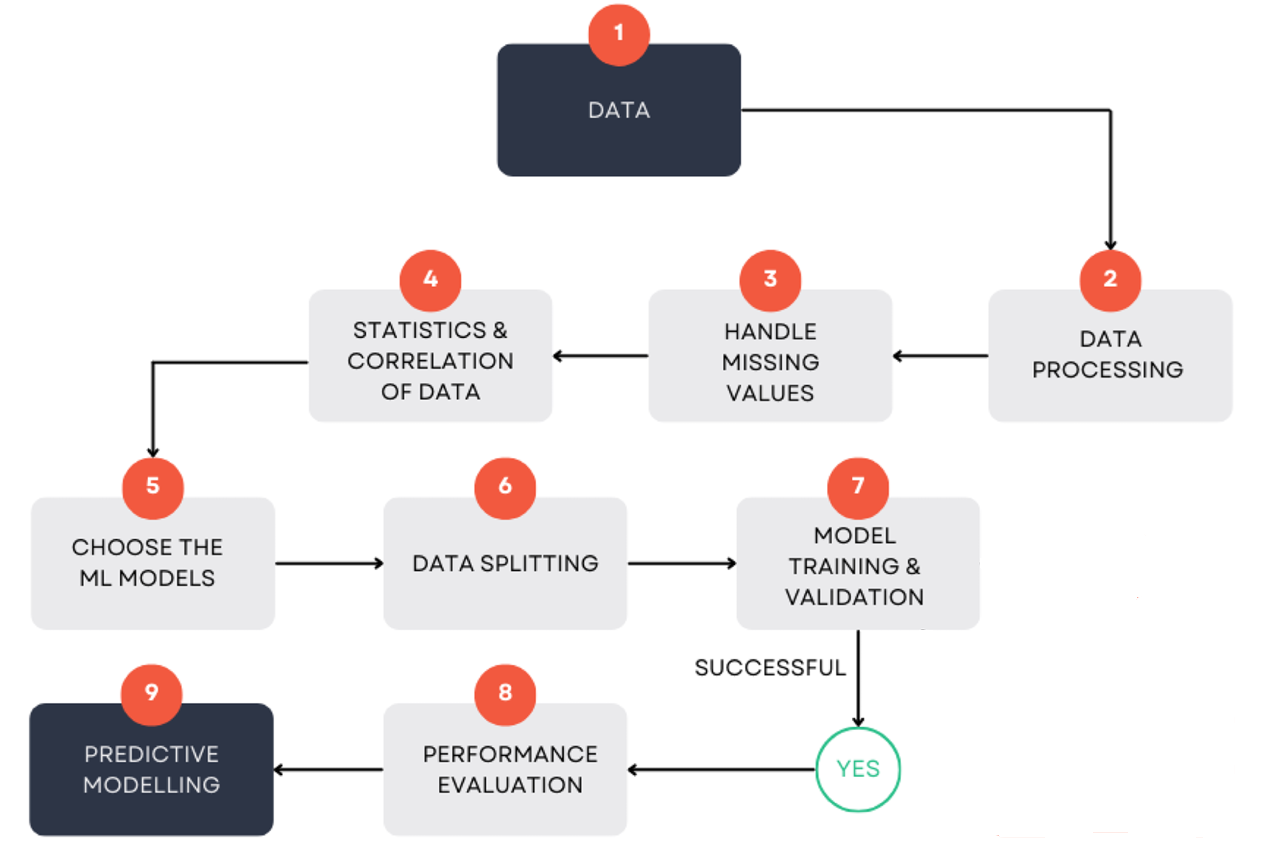
\includegraphics[width=\linewidth]{figures/DataFlow.png}
	\caption{Data collection and assessment algorithm for bearing failure prediction. Source: \cite{Dharmarathne2025}.}
	\label{fig:Dataflow}
\end{figure}
}
% Summary of FFT, data flow, etc.
\subsection{Signal Processing}
\subsubsection{Fourier Analysis}
{
In this section a deeper elabotation on Fourier Analysis and Transform is going to take place. 

Serafeimidou explains in detail the theoritical background of the Fourier Analysis \cite{diff_eq}. For an arbitrary finite range [-L,L] there is a family of functions, which meet the Dirichlet condition, and these functions can be expressed as a trigonometric sequence: 

\begin{equation}
    f(x) = \frac{a_0}{2} + \sum_{n=1}^{\infty} \left( a_n \cos(n\pi \omega x) + b_n \sin(n\pi \omega x) \right),
    \label{eq:tri_seq}
\end{equation}

where \( \omega = \frac{\pi}{L} \).

In addition its constants can be expressed as follows:

\begin{equation}
    a_n = \frac{1}{L} \int_{-L}^{L} f(u) \cos(n \omega u) \,du   
\end{equation}

\begin{equation}
    b_n = \frac{1}{L} \int_{-L}^{L} f(u) \sin(n \omega u) \,du    
\end{equation}

The equation \eqref{eq:tri_seq} needs to be expressed as a valid form within the whole \( x \in \mathbb{R} \). For this reason the  trigonometric integral (which is called Fourier integral) can be expressed as follows: 

\begin{equation}
    F(x) = \int_0^{\infty} \left[ A(\omega) \cos(\omega x) + B(\omega) \sin(\omega x) \right] \, d\omega
    \label{eq:tri_int}
\end{equation}

where: 
\begin{equation}
    A(\omega) = \frac{1}{\pi} \int_{-\infty}^{\infty} f(u) \cos(\omega u) \,du
    \label{eq:Aomega}
\end{equation}

\begin{equation}
    B(\omega) = \frac{1}{\pi} \int_{-\infty}^{\infty} f(u) \sin(\omega u) \,du
    \label{eq:Bomega}
\end{equation}

Assuming that there exist real functions \( f(x) \) defined in \( \mathbb{R} \) meeting the following points: 
\begin{itemize}
{
    \item \( f(x) \) and its derivative \( f'(x) \) are continuous in the range \( [-L, L] \subset \mathbb{R} \).
    \item \( f(x) \) is integrable in \( \mathbb{R} \):
	\[
    \int_{-\infty}^{\infty} |f(x)| \,dx < \infty.
    \]
}
\end{itemize}

Hence, given that the aforementioned conditions are met, \( A(\omega) \) (see Eq. \eqref{eq:Aomega}) and \( B(\omega) \) (see Eq. \eqref{eq:Bomega}) tend to attain a real value for \( \omega \), which implies that \( A(\omega) \) and \( B(\omega) \) are defined for every \( \omega \in \mathbb{R} \). In addition to this, the integral of the equation \eqref{eq:tri_int} tends to attain a real value for x, which ensues that F(x) is defined for every \( x \in \mathbb{R} \).

\( F(x) \) is identical to \( f(x) \) whenever \( f(x) \) is a continuous function. 
There are some special cases when \( f(x) \) is not a continuous function, and to deal with these cases, we define:

\begin{equation}
    F(x) = \frac{1}{2} \left[ \lim_{x \to x^+} f(x) + \lim_{x \to x^-} f(x) \right]
\end{equation}

This ensures that \( F(x) \) is properly handled even in cases of discontinuity.

All things considered the Fourier Transform \( F(\omega) = \mathcal{F} \{ F(x) \} \) can be mathematically expressed as follows:


\begin{equation}
    F(\omega) = \int_{-\infty}^{\infty} f(t) e^{-i \omega t} \,dt
\end{equation}


where the frequency can derive from the following form: \( \omega = \frac{2\pi j k}{N} \).

In practice, the Discrete Fourier Transform (DFT) boasts an extremely wide variety of applications, facilitating the Fourier Transform when applied to sampled signals. 

Hence, the mathematical formulation for determining the amplitude of each frequency, given a waveform \( x_0, x_1, \dots, x_{n-1} \) consisting of real values, is structured as follows:

\begin{equation}
    X(j) = \sum_{k=0}^{n-1} x(k) e^{ - \frac{i 2\pi jk}{n/2} }, \quad \text{for } j = 0,1,\dots,n-1.
    \label{eq:DFT}
\end{equation}
}
\subsubsection{Fast Fourier Transform (FFT)}
{
The Fast Fourier Transform (FFT) is an efficient algorithm for computing the Discrete Fourier Transform (DFT), expessed by the equation \eqref{eq:DFT} and its inverse. One of the most prominent FFT algorithms, the Cooley-Tukey algorithm \cite{CooleyTukey1965}, employs a divide-and-conquer approach to reduce the computational complexity from $\mathcal{O}(n^2)$ (for the naive DFT) to $\mathcal{O}(2 n \log n)$, enabling significant speedups for large amount of data.

This reduces complexity from $\mathcal{O}(n^2)$ (naive DFT entails direct implementation of the equation \eqref{eq:DFT}) to less than $\mathcal{O}(2 n \log n)$ (a Fast Fourier Transform implementation), enabling major time savings for complex and large-scale transforms. It is also worth articulating that the complexity can be interpreted as the number of operations executed \cite{CooleyTukey1965}, \cite{Singeleton1967}. 

Both algorithms are implemented in major numerical packages including MATLAB and NumPy's routines \cite{FFT}. What is highlighted  by Singeleton is that the Cooley-Tukey approach is considerably faster and decently performing especially when coupled with some additional practices so as to execute the Fast Fourier Transform \cite{Singeleton1967}. 

The computation time according to the aforementioned article decreases drastically by making use of the Cooley-Tukey algorithm. In addition, this very algorithm performs and adapts better to different applications compared to Good's, Danielson's and Goertzel's approaches.

Cooley and Tukey proved that the sample length can be composite size where it is preferable to make use of sample points sized as power of 2, especially when it comes to personal computers with binary arithmetic system. In addition to this the authors have proven that the power of 3 is formally the most efficient approach, however in the context of the fast Fourier Analysis the so-called Radix-2 implementation is the prominent one \cite{CooleyTukey1965}.

\begin{equation}
	N = 2^m \label{eq:radix_condition}
\end{equation} 

It is hereby worth it elaboration on the Fast Fourier Transform algorithm \cite{CooleyTukey1965}. The indices of the equation \eqref{eq:DFT} can be expressed as follows: 

\begin{equation}
	\begin{aligned}
		j &= j_{m-1} \cdot 2^{m-1} + j_{m-2} \cdot 2^{m-2} + \dots + j_1 \cdot 2 + j_0, \\
		k &= k_{m-1} \cdot 2^{m-1} + \dots + k_1 \cdot 2 + k_0,
	\end{aligned}
\end{equation}

where \( j_{v} \) and \( k_{v} \) are the contents of the respective bit positions within the binary representation, which ensues that they are equal to 0 or 1.

The aforementioned set-up (see eq. \eqref{eq:DFT}) leads to the following equation \eqref{eq:FFT}, encompassing twiddle factors expressed as:

\begin{equation}
	W = e^{-2\pi i/N}
	\label{eq:twiddle}
\end{equation}

And the Fast Fourier Transform:

\begin{equation}
	X(j_{m-1}, \cdots ,j_0) = \sum_{k_{0}} \sum_{k_{1}} \cdots \sum_{m-1} x({k_{m-1} , \cdots , k_0}) \cdot W^{j \cdot k_{m-1} \cdot 2^{m-1} + \cdots + j \cdot k_0}
	\label{eq:FFT}
\end{equation}

where as per the first step:
\begin{equation}
	W^{j \cdot k_{m-1} \cdot 2^{m-1}} = W^{j_{0} \cdot k_{m-1} \cdot 2^{m-1}}
\end{equation}

Furthermore, in the context of the first calculation, the first array can be expressed as follows:

\begin{equation}
	x_{1}(j_0, k_{m-2}, \cdots, k_0) = \sum_{\mathbf{k_{m-1}}} x(\mathbf{k_{m-1, \cdots, k_0}}) \cdot W^{\mathbf{j_0}  \cdot \mathbf{k_{m-1}} \cdot \mathbf{2^{m-1}} }
\end{equation}

And hereunder can be contemplated that proceeding to the next innermost-successive sum:

\begin{equation}
	W^{j \cdot k_{m-1} \cdot 2^{m-1}} = W^{(j_{l-1} \cdot 2^{l-1} + \cdots + j_0) \cdot k_{m-l} \cdot 2^{m-l}}
\end{equation}

followed by the calculation of the arrays:

\begin{equation}
	x_{l}(j_0, \cdots, j_{l-1} , k_{m-l-1} , \cdots, k_0) = \sum_{\mathbf{k_{m-l}}} x_{l-1}(j_0, \cdots , j_{l-2} \cdots, k_{m-l} , \cdots , k_0) \cdot  W^{(j_{l-1} \cdot 2^{l-1} + \cdots + j_0) \cdot k_{m-l} \cdot 2^{m-l}}
	\label{eq:Radix2}
\end{equation}

for l = 1, 2, ... , m

And this could constitute a recursive procedure obtaining the successive arrays. And last but not least, this finally could lead to the calculation of X spectrum. It can be contemplated that from the Equation \eqref{eq:Radix2}, there is at all times two consecutive values, the even and the odd value that can be stored at a specific location corresponding to an index of: 

\begin{equation}
	(j_0 2^{m-1} + \cdots + j_{l-1} 2^{m-l} +  k_{m-l-1} 2^{m-l-1} + \cdots + k_0)
\end{equation}

It is also worth it recalling that m is defined by \( N = 2^m \). Since bit positions \( 2^(m-l) \), meaning the j and k coefficients, can only get the values 0 and 1, which ensues that there is multiple-storage locations that can be calculated simultanously.

The array calculated gives the desired Fourier sums: 

\begin{equation}
	X(j_{m-1}, cdots, j_0) = A_{m}((j_0 , cdots , j_{m-1})
\end{equation}


At this point there is a need to simplify the Fast Fourier Transform algorithm. It is mendatory to recall the \eqref{eq:FFT} so as to depict the algorithm. 

The calculations workload can be reduced, by decomposing the original input sequence \( X[k] \), of length \( N \), into two subsequences:

\begin{itemize}
    \item A sequence consisting of elements at even-numbered indices: \( X_{\text{even}}[k] \)
    \item A sequence consisting of elements at odd-numbered indices: \( X_{\text{odd}}[k] \)
\end{itemize}

By processing these smaller sequences independently, the algorithm substantially reduces the computational workload. The FFT is applied recursively to each half, and this decomposition continues until each subproblem has length 1, at which point the computation becomes trivial (the amplitude value corresponding to a specific frequency). Furthermore, the results from the smaller FFTs are recombined using twiddle factors (see Equation \eqref{eq:twiddle}).

An significant property of this algorithm is that that, in the case of \( j > \frac{n}{2} \), the values are repeated due to the sinusoidal property of \( \exp \), which is known as the symmetry identity. This entails that for the values \( j = 0,1,\dots,n/2-1 \):

\begin{equation}
	X_{\text{even}}(j + n/2) = X_{\text{even}}(j) \quad \text{and} \quad X_{\text{odd}}(j + n/2) = X_{\text{odd}}(j)
	\label{eq:Sym}
\end{equation}


The evens and odds decomposition:
\begin{equation}
    X_{even}(j) = \sum_{k=0}^{n/2-1} x(2k) e^{ - \frac{i 2\pi jk}{n/2} }, \quad \text{for } j = 0,1,\dots,n/2-1.
    \label{eq:Xeven}  
\end{equation}

\begin{equation}
    X_{odd}(j) =  \sum_{k=0}^{n/2-1} x(2k+1) e^{ - \frac{i 2\pi jk}{n/2} }, \quad \text{for } j = 0,1,\dots,n/2-1.
    \label{eq:Xodd}
\end{equation}

So from the Equation \eqref{eq:FFT}:
\begin{equation}
    X(j) =  X_{even}(j) + e^{- \frac{i 2\pi j}{n}} X_{odd}(j)
    \label{eq:expterm}
\end{equation}

And this procedure is scalable since each and every \( X_{even} \) and \( X_{odd} \) can be deplited into a subsequent set of \( X_{eve} \) and \( X_{odd} \) to the point that the length 1 is reached.

Last but not least, the symmetry identity as described by the Equation \eqref{eq:Sym}, leads to the following set of equations (see also \eqref{eq:expterm}):

\begin{equation}
    X(j+n/2) =  X_{even}(j) + e^{- \frac{i 2\pi (j+n/2)}{n}} X_{odd}(j)
\end{equation}

For the values \( j = 0,1,\dots,n/2-1 \).

The objective of this algorithm is to get to the point that the length is of the sums is 1, meaning that the sums of the Equations \eqref{eq:Xeven} and \eqref{eq:Xodd} are applicable for k=0. The only  remaining exponential terms  \( e^{- \frac{i 2\pi j}{n}} \) in the Equation \eqref{eq:expterm} - as previously described by Equation \eqref{eq:Radix2}.

The aforementioned procedure can be further repeated, by breaking the branches problem into sub-branches. The radix-2 DIT algorithm to be formulated as follows on Figure \ref{fig:RecFFT}, depicting the concept of narrowing down the problem. 

\begin{figure}[h]
    \centering
    \begin{tikzpicture}

        % Level 0
        \node[draw, rectangle] (X) at (0,0) {Input \( X[0 \dots] \)};

        % Level 1
        \node[draw, rectangle] (Xe) at (-4,-2) {\( X_{\text{even}} \)};
        \node[draw, rectangle] (W) at (3,-2) {\( W \)};
        \node[draw, rectangle] (Xo) at (4,-2) {\( X_{\text{odd}} \)};
        \draw[->] (X) -- (Xe);
        \draw[->] (X) -- (Xo);

        % Level 2
        \node[draw, rectangle] (Xee) at (-6,-4) {\( X_{\text{even}} \)};
        \node[draw, rectangle] (W) at (-3,-4) {\( W \)};
        \node[draw, rectangle] (Xeo) at (-2,-4) {\( X_{\text{odd}} \)};
        \node[draw, rectangle] (Xoe) at (2,-4) {\( X_{\text{even}} \)};
        \node[draw, rectangle] (W) at (5,-4) {\( W \)};
        \node[draw, rectangle] (Xoo) at (6,-4) {\( X_{\text{odd}} \)};
        \draw[->] (Xe) -- (Xee);
        \draw[->] (Xe) -- (Xeo);
        \draw[->] (Xo) -- (Xoe);
        \draw[->] (Xo) -- (Xoo);

        % Ellipsis (continued decomposition)
        \node at (-6,-5.5) {\dots};
        \node at (-2,-5.5) {\dots};
        \node at (2,-5.5) {\dots};
        \node at (6,-5.5) {\dots};

    \end{tikzpicture}
    \caption{Recursive decomposition using even-odd splitting.}
    \label{fig:RecFFT}
\end{figure}

All in all, this section yields an overview of utmost importance highlighting the most invaluable Fourier Transform algorithms expressed by equation \eqref{eq:DFT} and equation \eqref{eq:FFT}.
As discussed in this section, the Cooley-Tukey Fast Fourier Transform (FFT) algorithm significantly accelerates the computation of the Discrete Fourier Transform (DFT) by recursively breaking the problem into smaller, more manageable subproblems. This divide-and-conquer approach is fundamental to the algorithm’s performance advantage.

}



\subsection{Internet of Things} 
{
	\subsubsection{Introduction to Internet of Things \& Key Technologies}
	{
		The ultimate objective of this project is to create a set-up that is well-rounded and has a real-time monitoring and assessment competency. Two of the most prominent technologies that are being incorporated by Internet of Things (IoT) is the cloud computing and the wireless communication. It is also worth mentioning that, Internet of things encompasses interconnection of physical devices and applicaitons making the most of sensors, networks and data analysis. 
	}
	
	\subsubsection{Cloud-Oriented Perspective \cite{Gubbi2013}}
	{
		An extremely accurate definition of the \textit{Internet of Things} is given by Gubbi et al, articulating that:
		
		\begin{quote}
			``Interconnection of sensing and actuating devices providing the ability to share information across platforms through a unified framework, developing a common operating picture for enabling innovative applications. This is achieved by seamless ubiquitous sensing, data analytics and information representation with Cloud computing as the unifying framework.''
		\end{quote}
		
		This approach is mostly "Cloud"-oriented. The authors focus mostly on the concept of ubiquitous information and evolving communication networks. The means to give ground to this very concept is Smart Connectivity. It is fueled by the prevalence of devices enabled by open wireless technology such as Bluetooth, radio frequency identification (RFID), Wi-Fi, and telephonic data services as well as embedded sensor.
		
		Nevertheless, Hardware-sensor breakouts are critically important, as they serve as the primary means of data collection in IoT systems. Middleware and computing tools for data analytics are equally invaluable, as they enable the processing of raw sensor data into actionable insights. Finally, visualization tools and dashboards play a key role in end-user interaction with the IoT environment, while also providing stakeholders with an intuitive and accessible representation of the data \cite{Gubbi2013}.
	}
	
	\subsubsection{Internet- vs. Things-Oriented Perspectives \cite{Atzori2010}}
	{
		As regards the approach of Atzori et al, there is given a different definition by considering two different approaches, the "Internet"-oriented approach and the "Things"-oriented approach. The "Things"-oriented approach targets mainly at Big Data applications, since according to Atzori et al the time, the place and multipe recipients are the most important factors of this approach. In essnece the "Things" that contribute to this perspective are the Radio-Frequency IDentification (RFID), Near Field Communications (NFC) and Wireless Sensor and Actuator Networks (WSAN) among others.
		
		The "Internet"-oriented vision given by Atzori et al, it is highlighted that the IP (Internet Protocol) constitutes the core technology of Internet of Things (IoT). The Internet Protocol (IP) is lightweight, scalable, and capable of connecting smart objects worldwide—even on low-power devices. The authors also introduce Internet Ø, a similar approach that further simplifies IP to enable "IP over anything," ensuring seamless IoT integration. The ultimate goal of both strategies is to make all objects addressable, reachable, and interoperable through IP, moving from a basic "Internet of Devices" to a fully connected "Internet of Things" \cite{Atzori2010}. 
	}
	
	\subsubsection{Semantic-Oriented Approach}
	{
		In addition to the aforementioned perspectives there is an emerging need for representation and storage of the invaluable information, which leads to the "Semantic"-oriented approach (see \ref{fig:IoT}). This final approach creates a well-rounded Internet of Things (IoT) concept, yielding more details on it. 
		
		The whole concept of the vast majority of different projects requires a semantic approach so as to set some thresholds and yield some feedback or take some action over something. In addition to this the semantic vision according to Atzori et al expresses the need for a representation of the collected data \cite{Atzori2010}.
		
		\begin{figure}[h]
			\centering
			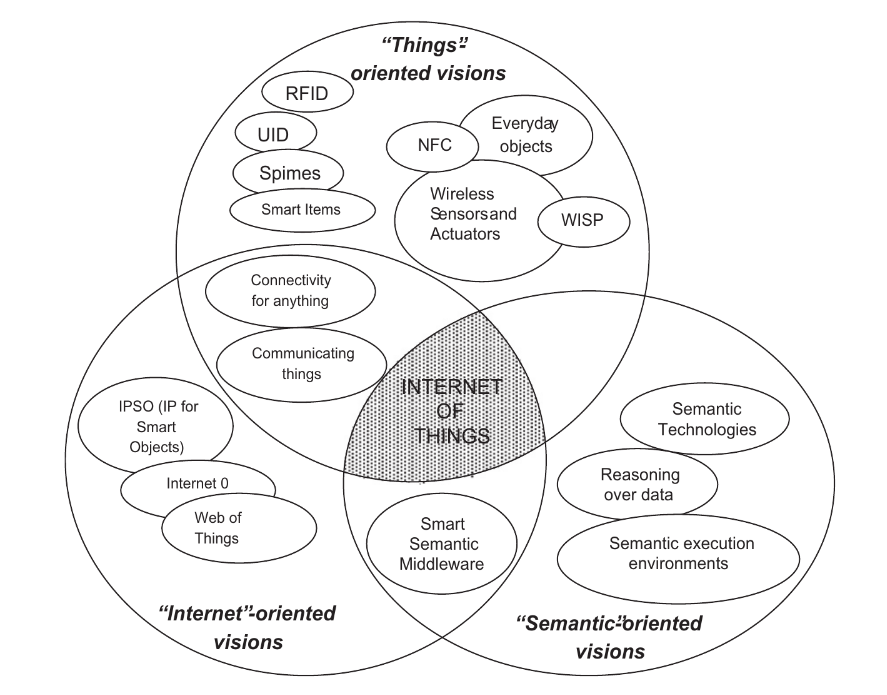
\includegraphics[width=\linewidth]{figures/IoT.png}
			\caption{The Internet of Things paradigm as a result of the convergence of different visions. Source: \cite{Atzori2010}.}
			\label{fig:IoT}
		\end{figure}
			
		All in all Atzori defines Internet of Things (IoT) as follows:
			\begin{quote}
				``Internet of Things constitutes a world-wide network of interconnected objects uniquely addressable, based on standard communication protocols.``
			\end{quote}
		}
		
		
		
		
		
		
		
	\subsubsection{Project Implementation: Sensing \& Communication}
	{
As it has been highlighted by the Internet of Things definitions, the sensors are among the most important devices of this technology. The sensing unit in this project utilizes an ADXL335 accelerometer to collect physical acceleration data, which connects to the microcontroller through an analog input interface. 
		
Its operational principles can be summarized as follows \cite{ADXL335}:

\paragraph{Sensing Mechanism}
\begin{itemize}
	\item Utilizes a surface-micromachined polysilicon structure suspended by springs 
	\item Employs a differential capacitor design with:
	\begin{itemize}
		\item Fixed plates driven by 180° out-of-phase square waves
		\item Moving plates attached to the proof mass
	\end{itemize}
	\item Acceleration causes proof mass deflection, unbalancing the capacitor
	\item Phase-sensitive demodulation determines acceleration magnitude/direction
\end{itemize}

\paragraph{Key Features}
\begin{itemize}
	\item \textbf{Monolithic Construction}: Single structure for X/Y/Z axes ensures:
	\begin{itemize}
		\item High orthogonality ($<$1\% cross-axis sensitivity)
		\item Temperature stability ($<$3mg hysteresis from -25°C to +70°C)
	\end{itemize}
	\item \textbf{Signal Conditioning}:
	\begin{itemize}
		\item On-chip 32k$\Omega$ output resistor
		\item User-adjustable bandwidth (0.5-1600Hz via external capacitors)
	\end{itemize}
	\item \textbf{Power Management}:
	\begin{itemize}
		\item Basic decoupling: 0.1$\mu$F capacitor near supply pins
		\item Enhanced noise rejection: 100$\Omega$ ferrite bead + 1$\mu$F bulk capacitor 
	\end{itemize}
\end{itemize}

\paragraph{Measurement Capabilities}
The device measures both:
\begin{itemize}
	\item Static acceleration (e.g., tilt sensing through gravity detection)
	\item Dynamic acceleration (vibration, shock, motion)
\end{itemize}

This combination of mechanical design and signal processing provides robust acceleration measurement without requiring temperature compensation circuits or complex calibration procedures \cite{ADXL335}.
		
		The system architecture supports multiple communication protocol options, each with distinct advantages:
		
		\begin{itemize}
			\item \textbf{Analog Input}: Currently implemented for direct sensor interfacing (ADXL335)
			\item \textbf{Digital Input}: Available for threshold-based detection applications
			\item \textbf{SPI (Serial Peripheral Interface)}: Suitable for high-speed (up to 10 Mbps) communication with multiple peripherals
			\item \textbf{I\textsuperscript{2}C (Inter-Integrated Circuit)}: Enables multi-device communication using only two wires (SDA/SCL)
			\item \textbf{UART (Universal Asynchronous Receiver-Transmitter)}: Implemented at 9600 baud (8N1 format) for Arduino-to-Raspberry Pi communication
		\end{itemize}
		
		The UART protocol was specifically selected for inter-processor communication due to:
		\begin{itemize}
			\item Native hardware support on both Arduino and Raspberry Pi platforms
			\item Simplified point-to-point implementation
			\item Sufficient bandwidth for the project's real-time data transmission needs
		\end{itemize}
		
		This hybrid approach combining analog sensor interfacing with digital serial communication provides optimal balance between:
		\begin{itemize}
			\item Signal fidelity at the sensing stage
			\item System-wide data reliability
			\item Implementation efficiency
		\end{itemize}
	}
 
 
 
	 
	 
	\subsection{Embedded System Design} 
	{
		\subsubsection{Sensor Layer: ADXL335 Accelerometer}  
		The ADXL335 is a 3-axis accelerometer that measures acceleration using analog voltage outputs. This section discusses its interfacing with an Arduino and signal processing.  
		
		\begin{itemize}  
			\item \textbf{Sensor Breakout Board}  
			A breakout board simplifies the connection of the ADXL335 by providing necessary components (e.g., voltage regulation, filtering capacitors) and standardized pin headers. This avoids the need for complex PCB design when prototyping.  
			
			\item \textbf{Analog Signal Transmission}  
			The ADXL335 outputs analog voltages proportional to acceleration. Unlike digital signals (discrete values), analog signals are continuous and susceptible to noise. The Arduino's ADC (Analog-to-Digital Converter) reads these voltages for processing.  
			
			\item \textbf{Signal Conditioning \& Processing}  
			Since analog signals degrade over long wires, techniques like filtering (RC low-pass) and amplification may be needed. Calibration (mapping voltage to g-forces) is also essential for accurate readings.  
		\end{itemize}
		
		\subsubsection{Microcontroller: Arduino}  
		\begin{itemize}  
			\item \textbf{UART Protocol}: 9600 baud, 8N1 frame format.  
			\item \textbf{Data Relay}: Reads ADC, sends CSV string via serial.  
		\end{itemize}  
		
		\subsubsection{Gateway: Raspberry Pi 4}  
		\begin{itemize}  
			\item \textbf{UART-to-HTTP Bridge}:  
			\begin{enumerate}
				\item Python script reads serial port.  
				\item Formats JSON payload.  
				\item POSTs to Supabase API.  
			\end{enumerate}
		\end{itemize}  
		
		\subsubsection{Backend: Supabase \& Vercel}  
		\begin{itemize}  
			\item \textbf{Supabase}: PostgreSQL tables with time-series data.  
			\item \textbf{Vercel}: Hosts Next.js dashboard fetching Supabase data.  
		\end{itemize}  
	}
	 
